%!TEX root = ../main.tex
% !TeX spellcheck = en_GB 


\chapter{Implementation}
The objective of this thesis was to implement and evaluate a  collision avoidance  algorithm for USVs. Several related approaches where analysed before the fuzzy logic approach presented by \textcite{perera2012intelligent}, was chosen to be implemented.
The solution presented in the original paper is implemented in MATLAB, while the solution presented here is implemented in Python. Python was chosen due to the writers previous knowledge of the language as well as the availability of fuzzy logic python libraries. The library used in this implementation is called SciKit-Fuzzy \cite{josh_warner_2017_1002946}.

\section{The fuzzy inference system}
The fuzzy logic framework SciKit-Fuzzy is used to implement the model described in section \ref{section:model}. The framework provides a simple API which enables one to define Antecedents, Consequents, their corresponding FMFs as well as the rules that unite them.

First antecedents are initialized as shown in listing \ref{listing:ant}.
\begin{listing}[ht]
    \begin{minted}{python}
bear = ctrl.Antecedent(np.arange(0, 360, 1), 'bearing')
\end{minted}
    \caption{Antecedent initialization}
    \label{listing:ant}
\end{listing}
This example creates the antecedent \textit{bearing} with a universe spanning from 0 to 360 with steps of 1. FMFs are then added to the antecedent. Listing \ref{listing:fmf} shows the FMF for sector II of the model. It starts at 5\textdegree relative bearing and ends at 85\textdegree, with a 5 \textdegree  fuzziness on both sides.
\begin{listing}[ht]
    \begin{minted}{python}
bear['2'] = fuzz.trapmf(bear.universe, generate_trapetzoid(5, 85, 5))
\end{minted}
    \caption{FMF initialization}
    \label{listing:fmf}
\end{listing}

The other antecedents and consequents are initialized and populated with FMFs in the same manner, according to the model described in section \ref{section:model}.

Rules are defined in order to connect the antecedents with consequents.
A rule consist of an antecedent and a consequent as follows:
\begin{minted}{python}
Rule(antecedent, consequent)
\end{minted}
Where the parameter \textit{antecedent} can be a combination of antecedents using the \textit{\&} and \textit{|} operators.
An example based on \ref{rule:1} in section \ref{section:FIS} can be seen in listing \ref{listing:rule}.
\begin{listing}[ht]{}
    \begin{minted}{python}
Rule(
    'II' &
    'f' &
    '>1' &
    ('Rvd'|'Ra'|'Rb'),
    'starboard','decrease')
            
\end{minted}
    \caption{Rule initialization}
    \label{listing:rule}
\end{listing}

These rules are then passed to the ControlSystem that each vessel utilizes to calculate proper course and speed corrections.
\section{Architecture}
This section will present the high level structure of the implementation with the help of the class diagram seen in figure \ref{fig:class_diagram}. Each class and their interactions will be briefly presented.
\begin{figure}[H]
    \centering
    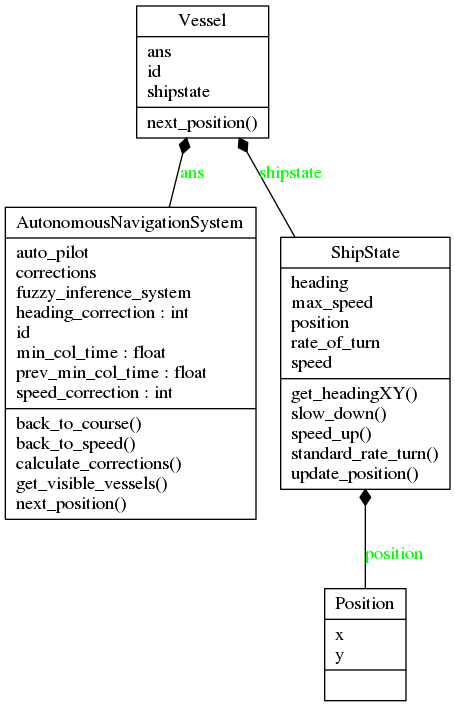
\includegraphics[width=\textwidth,height=0.75\textheight,keepaspectratio]{../src/classes_Pyreverse}
    \caption{Class diagram}
    \label{fig:class_diagram}
\end{figure}
\subsection{Classes}
Each simulation scenario consists of at least one vessel. These vessels are represented by the \textit{Vessel} class. The current state of the vessel is represented by the \textit{ShipState} class which also contains the \textit{Position} class. Furthermore, each vessel need a navigation system, which is represented by the \textit{AutonomousNavigationSystem} class. The classes will be more thoroughly presented in the following subsections.
\subsubsection{Vessel}
\textit{Vessel} is the main class and the class with which the simulation script interacts.
It contains, apart from the previously mentioned \textit{AutonomousNavigationSystem} and \textit{ShipState} an id and a method to calculate it's position in the next time frame.
A new vessel object in created with the following call:
\begin{minted}{python}
Vessel(id, heading, position_x, position_y, speed, max_speed, 
    rate_of_turn, fuzzy_inference_system, auto_pilot)
\end{minted}
This constructor call specifies the ID for the vessel as well as its initial position, speed and heading. Furthermore it defines the vessels maximum speed and rate of turn. The two final parameters specify the fuzzy inference system to use and whether the vessel shall use the navigation system. Setting the final boolean to false creates a rogue vessel that will just keep its initial speed and heading, thereby not complying to the COLREG rules. The \textit{Vessel} class has only one method, which calculates the vessels position in the next time frame after applying possible corrections to heading ans speed.
\subsubsection{Position}
The position class simply holds the vessels current coordinates in the Cartesian coordinate system used.
\subsubsection{ShipState}
ShipState holds information about the state of the vessel in the current time frame. This includes the vessels current position, heading and speed. The simulation does not distinguish between course and heading since no drift is simulated.
Furthermore, limits such as maximum allowed speed and standard rate of turn is specified in this class. Finally, the class holds methods to change the ships heading by the specified standard rate of turn or speed by 1 kt, for the next time frame.


\subsubsection{AutonomousNavigationSystem}
\label{sec:ANS}
The AutonomousNavigationSystem class from now on referred to as ANS is what separates an autonomous vessel from an ordinary vessel. The ANS combines the information from the ShipState class with situational awareness information provided by a separate Situational Awareness (SA) module, in order to calculate needed corrections to speed and course.

The SA is in this simulation case represented by a service that holds all information regarding the current scenario. A real system would have a SA module that reads and processes information from different sensors, such as LiDAR, cameras, on board the vessel. Information needed about a target vessel is its heading, speed, and position. These are used to calculate the four different inputs to the FIS system. Listing \ref{listing:rel_bear_calc} shows the method used to calculate the relative bearing fed into the FIS system. Compass bearing is first calculated from the two provided coordinate pairs after which the result is converted into a relative bearing. Relative course is then calculated as the observed vessels heading - the own vessels heading, as shown in listing \ref{listing:rel_course_calc}. Distance can be obtained by using the Pythagorean theorem on the differences between the vessels in the X and Y axis. Finally speed ratio is defined as $\frac{\text{Speed of the observed vessel}}{\text{Speed of the own vessel}}$.
\begin{listing}

    \begin{minted}[linenos, breaklines=true,fontsize=\scriptsize, numberblanklines=false]{python}
rel_course = observed_vessel.shipstate.heading - shipstate.heading
if rel_course < 0:
    rel_course = 360 + rel_course
    \end{minted}
    \caption{Relative course calculation}
    \label{listing:rel_course_calc}
\end{listing}

These inputs are fed into the FIS system, for each target vessels, and the recommended corrections are stored in an array. The recommendations might however contradict each other and a way to prioritize the recommendations is therefore needed.

Furthermore the expected time until collision needs to be calculated for each target vessel to prioritize the recommended corrections. Knowing the distance between the vessels, their relative velocity is needed to calculate the time. Equation \ref{eq:rel_vel_calc} shows the relative velocity calculation, based on the law of Cosines. \textit{V} stands for velocity, $\theta$ for heading, the subscript \textit{m} for own vessel and \textit{t} for target vessel.

\begin{equation}
    V_r=\sqrt{V_m^2 + V_t^2-2  V_mV_tcos(\theta_m-\theta_t)}
    \label{eq:rel_vel_calc}
\end{equation}

The previous calculations results in speed and heading correction suggestions, as well as an expected time until collision, for each target vessel. However, these recommendations might contradict each other and a way to prioritize the corrections in order of urgency is therefore needed. This is in this implementation solved in a simple matter by calculating the weighted arithmetic mean of the corrections using the expected time until collision as weight. The resulting corrections are then stored in ShipState as target heading.

Finally the heading and speed of the vessel is updated in the following manner. The vessels is steered towards the proposed heading change by a maximum of the vessels defined maximum rate of turn. The speed is similarly changed towards the proposed speed by a maximum of one knot. No proposed correction by the FIS means that the vessel is currently not in a scenario satisfies a rule in the rule set. However, a previous correction suggestion might still not be completed due to the vessels limited rate of turn, acceleration or deceleration.  The vessel will therefore continue to change its heading and speed towards the saved target speed until they are the same.  The target heading is then gradually changed towards the original heading until the vessel is back on its original heading. The process is visualized in Figure \ref{fig:flow_chart}.
\begin{figure}[H]
    \centering
    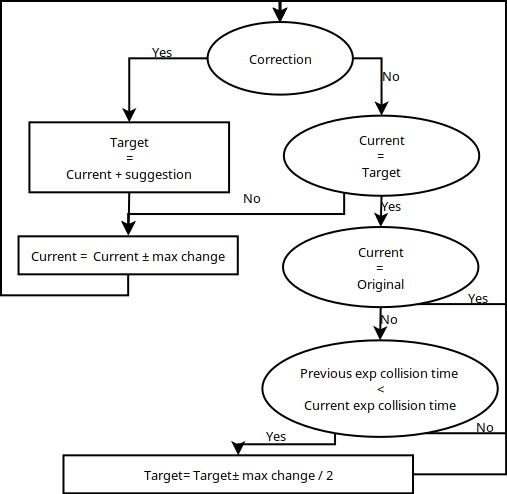
\includegraphics[width=\textwidth,height=0.75\textheight,keepaspectratio]{Figures/flow.png}
    \caption{Flow chart explaining application of heading and speed corrections}
    \label{fig:flow_chart}
\end{figure}

\section{Simulation}
The goal of the implementation is to  simulate a real world situation with respect to time, speed, acceleration, and rate of turn, while neglecting  environmental factors such as weather.
The simulation is therefore limited to two dimensions in a Cartesian coordinate system.
The interval between time frames in the simulation is set to correspond to one second in the real world.
Each iteration of the main simulation loop must, therefore, update the vessels SA by scanning the environment for target vessels. The information gained is then fed into the FIS which generates course and speed corrections which is used to update heading and speed as explained in section \ref{sec:ANS}.
\chapter{Scenarios}
\label{sec:overtaking-and-head-on}
Three scenarios are defined in order to test the ANS in multi vessel situations. Ideas for the scenarios are from \textcite{ecolreg_overtaking-and-crossing-2,ecolreg_overtaking-and-crossing-3,ecolreg_overtaking-and-crossing,ecolreg_overtaking-and-head-on}, with a few minor modifications. All scenarios are set in high visibility on the high sea.
\section{Overtaking and head-on situation}
The first scenario defines a three vessel situation, where two vessels are meeting on a reciprocal course. One of the vessels is, furthermore, overtaking a third ,vessel on the stand on vessels starboard side. A visualization of the scenario is shown in figure \ref{fig:overtaking-and-head-on}. Vessels \textit{A} and \textit{B} starts on reciprocal tracks 20 NM from each other, while \textit{B} and \textit{C} starts abreast 2 NM from each other. \textit{A}, \textit{B}, and \textit{C} has an max speed of 15 kts. \textit{A} and \textit{B} starts at 12 kts while \textit{C} is slightly slower at 10 kts. Max rate of turn of all vessels is set to 3\textdegree/second. The numbers on the vessels tracks helps to compare the vessels positions at a given time frame.

Vessels \textit{A} and \textit{B} are therefore obliged to alter their courses to starboard to prevent a head on collision (\textit{Rule 14}). Moreover vessel \textit{B} shall keep out of the way of \textit{C}  and in no circumstance alter its course so that it becomes a crossing vessel to \textit{C} (\textit{Rule 13}). All corrections shall furthermore be ample, so that it is recognizable by the other vessel, and taken as early as possible (\textit{Rule 16}) \cite{ecolreg_overtaking-and-head-on}.
\begin{figure}[H]
    \centering
    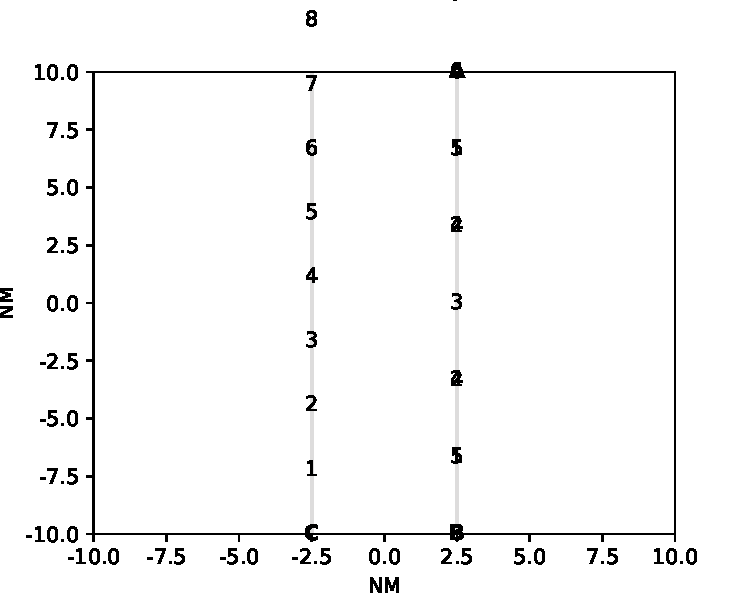
\includegraphics[width=\textwidth,height=0.75\textheight,keepaspectratio]{Figures/Scenario/overtaking-and-head-on.pdf}
    \caption{Overtaking and head-on situation on the high seas  \cite{ecolreg_overtaking-and-head-on}}
    \label{fig:overtaking-and-head-on}
\end{figure}



\section{Overtaking and crossing situation}
The following three scenarios both depict situations where vessels \textit{A} and \textit{B} is in an overtaking condition while \textit{C} crosses both their paths. \textit{C} crosses \textit{A} and \textit{B}s paths with a 45\textdegree  angle in the first scenario (figure \ref{fig:overtaking-and-crossing}). \textit{A} starts at (-6900, -7200), \textit{B} at (5100, -8000) and \textit{C} in origo. \textit{A} and \textit{B} has an initial heading of 0\textdegree  while \textit{C} start with a heading of 235\textdegree. The speeds of the vessels is set to ensure that \textit{C} would collide with both vessels if no corrections are applied. Moreover the speed of \textit{B} must be greater than the speed of \textit{A} since \textit{B} is overtaking \textit{A}. The vessels initial speed are, therefore: \textit{A} = 2kts, \textit{B} = 5.2kts and \textit{C} = 7.6kts. The maximum speeds of the vessels are 10, 15 and 20 kts respectively. Max rate of turn of all vessels is set to 3\textdegree/second.

Rule 13 and 16 applies to this scenario in the same way as the previous one, with the exception that the vessels involved in the overtaking situation is vessel \textit{A} and \textit{B} instead of \textit{B} and \textit{C}. This implies that \textit{B}shall keep out of way of \textit{A} (\textit{Rule 13}), while \textit{A} shall keep its course and speed (\textit{Rule 17}).

Additionally both \textit{A} and \textit{B} are crossing \textit{C} with a risk of collision. This means that \textit{A} and \textit{B} should alter their course to starboard and avoid passing in front of \textit{C} (\textit{Rule 15}). Vessel \textit{C} shall, meanwhile, keep its course and speed. This results in contradictory obligations for vessel  \textit{A}, where it should keep its course and speed for \textit{B} and simultaneously keep out of the way for vessel \textit{C}.

\textcite{ecolreg_overtaking-and-crossing} suggest the following manoeuvres for vessel \textit{A} and \textit{B} in accordance with the ordinary practice of seamen:
Both vessels might alter course to starboard and, thereby, pass behind vessel \textit{C}. Alternatively vessel \textit{A} may reduce speed or make a 360\textdegree turn to port, while vessel \textit{B} reduces speed, makes a 360\textdegree to starboard or alters its course to starboard.

\label{sec:overtaking-and-crossing}
\begin{figure}[H]
    \centering
    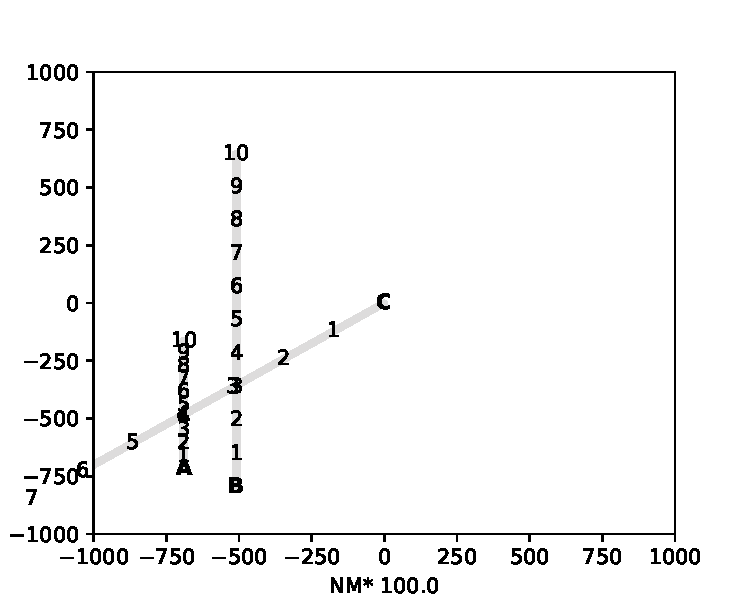
\includegraphics[width=\textwidth,height=0.75\textheight,keepaspectratio]{Figures/Scenario/overtaking-and-crossing.pdf}
    \caption{Overtaking and crossing situation on the high seas \cite{ecolreg_overtaking-and-crossing}}
    \label{fig:overtaking-and-crossing}
\end{figure}


\begin{figure}[H]
    \centering
    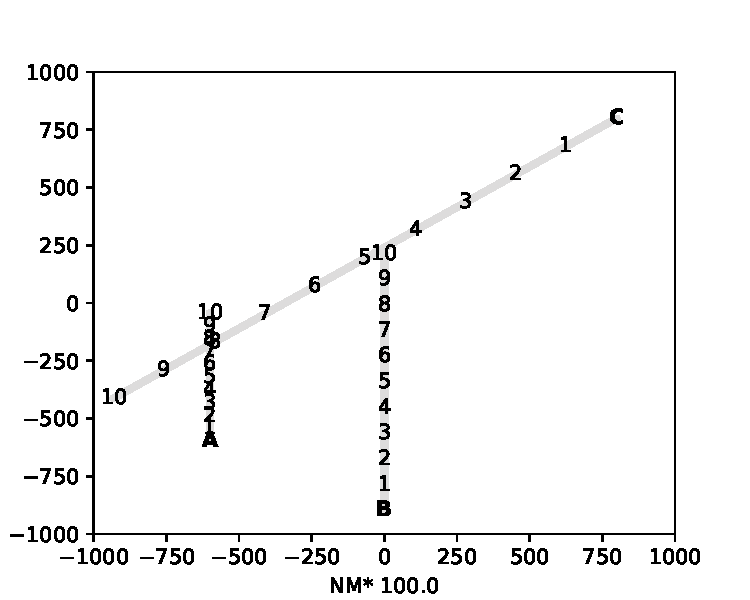
\includegraphics[width=\textwidth,height=0.75\textheight,keepaspectratio]{Figures/Scenario/overtaking-and-crossing-3.pdf}
    \caption{Overtaking and crossing situation\cite{ecolreg_overtaking-and-crossing-3}}
    \label{fig:overtaking-and-crossing-3}
\end{figure}


\begin{figure}[H]
    \centering
    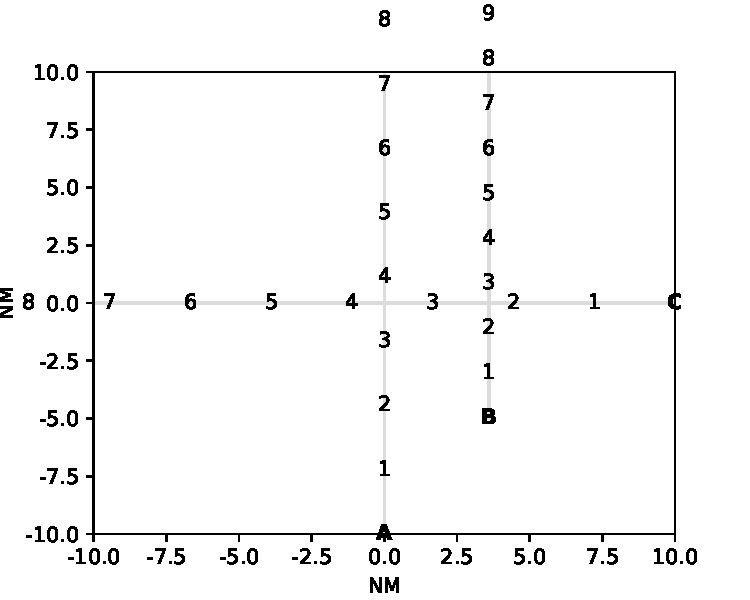
\includegraphics[width=\textwidth,height=0.75\textheight,keepaspectratio]{Figures/Scenario/overtaking-and-crossing-2.pdf}
    \caption{Overtaking and crossing situation\cite{ecolreg_overtaking-and-crossing-2}}
    \label{fig:overtaking-and-crossing-2}
\end{figure}
